\documentclass{beamer}

% 使用 ctexbeamer 文檔類來支援中文
\usepackage[UTF8]{ctex}
\usepackage{graphicx}
\usepackage{hyperref}
\usepackage{caption}
\usepackage{tabularx}
\usepackage{array}
\usepackage{amssymb}
\usepackage{amsmath}


% 移除圖表標題的前綴
\setbeamertemplate{caption}{\insertcaption}

% 主題設定
\usetheme{Madrid}
\usecolortheme{seagull}

% 標題信息
\title[TWSIAM 2025, 清華大學數學系]{AI For Math}
\author{作者名稱:簡偉恆、盧詠涵}
\institute[輔仁大學資數一]{輔仁大學\>\>數學系資訊數學組\>\>一年級}
\date{2025年6月8日}

\begin{document}

% 標題頁
\frame{\titlepage}

% 目錄頁
\begin{frame}
    \frametitle{大綱}
    \begin{enumerate}
        \item 社群活動簡介
        \item Kolmogorov–Arnold Network簡介
        \item Kolmogorov–Arnold Network實作
        \item 記憶模型是否能降低KAN的誤差
    \end{enumerate}
\end{frame}

% 第一節
\begin{frame}[c]{六堂課程總覽}
    \centering
    \textbf{113年學年度第二學期AI for Math系列演講}\\[0.1cm]
    \normalsize % 或 \scriptsize,依需要微調字體大小
    \begin{tabularx}{\textwidth}{%
        >{\centering\arraybackslash}p{1.8cm}  % 第一欄居中
        >{\centering\arraybackslash}p{1.6cm}  % 第二欄居中
        X         % 第三欄自動換行
    }
        \hline
        日期        & 講者    & \>\>\>\>\>\>\>\>\>\>\>\>\>\>\>\>\>\>\>\>\>\>\>\>\>\>\>\>\>\>\>\>\>\>\>\>\>\>\>\>\>講題 \\ \hline
        114/02/27   & 潘老師  & 感知機(The Perceptron) \\
        114/03/06   & 潘老師  & 淺談 Adaptive Linear Neuron 和 Widrow-Hoff Learning \\
        114/03/20   & 潘老師  & The Basics of Multilayer Perceptron and Backpropagation \\
        114/03/27   & 俞讚城 & Introduction to Shannon Entropy and Cross Entropy \\
        114/04/17   & 俞讚城 & Introduction to Universal Approximation Theorems and Application in AI \\
        114/05/08   & 嚴健彰 & KAN: Kolmogorov-Arnold Networks \\
        \hline
    \end{tabularx}
\end{frame}

\begin{frame}
    \frametitle{Kolmogorov–Arnold Network簡介}
    \centering
    \textbf{論文簡介}\\[0.5cm]
    \begin{itemize}
        \item 發表時間:2023年
        \item 標題:KAN: Kolmogorov–Arnold Networks
    %    \item 作者:Ziming Liu, Yixuan Wang, Sachin Vaidya, Fabian Ruehle, James Halverson, Marin Soljačić, Thomas Y. Hou, and Max Tegmark
        \item 主要特點:整合領域先驗知識與深度神經網路
        \item 應用領域:數學建模與科學計算
    \end{itemize}
\end{frame}

\begin{frame}
    \frametitle{Kolmogorov–Arnold Network簡介}
    \centering
    \textbf{MLP vs. KAN}\\
    \begin{figure}               % figure 環境(在 Beamer 中可省略,但如果要加 caption,就需要)
    \centering                 % 置中
    % \includegraphics[〈選項〉]{〈路徑/檔名〉}
    % 下面選項講解:
    %   width=0.8\textwidth    → 圖片寬度設定為投影片文字寬度的 80%
    %   keepaspectratio        → 保持原始比例(長寬比)
    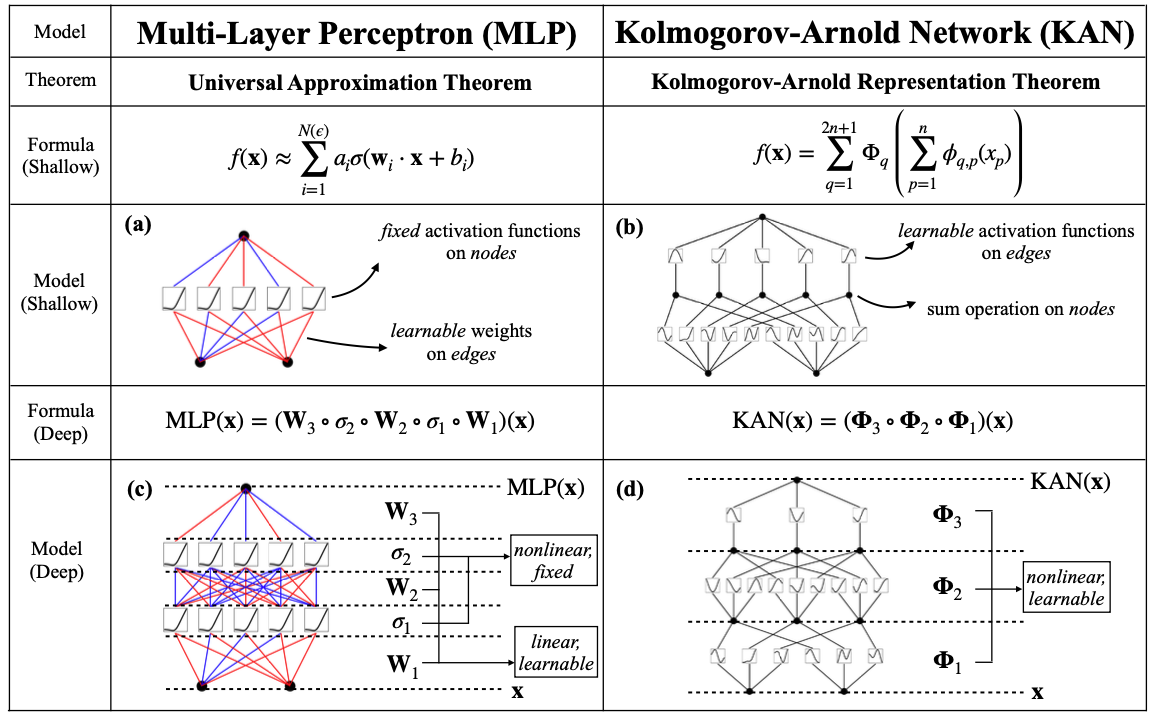
\includegraphics[width=0.9\textwidth,keepaspectratio]{figures/MLP_vs_KAN.png}
    \end{figure}
\end{frame}

\begin{frame}
    \frametitle{Kolmogorov–Arnold Network簡介}
    \centering
    \textbf{Kolmogorov–Arnold Networks 架構與特點}\\[0.5cm]
    \begin{itemize}
        \item Kolmogorov–Arnold Network(KAN)受Kolmogorov-Arnold Representation theorem(KAT)啟發
        \item 創新架構:
        \begin{itemize}
            \item 可學習的一維激活函數位於邊上,取代傳統線性權重
            \item 使用樣條函數(spline)參數化
            \item 每個節點僅執行線性加總,不附加任何非線性激活函數
        \end{itemize}
    \end{itemize}
\end{frame}

\begin{frame}
    \frametitle{Kolmogorov–Arnold Network簡介}
    \centering
    \textbf{Kolmogorov–Arnold Networks 架構圖}\\
    \begin{figure}               % figure 環境(在 Beamer 中可省略,但如果要加 caption,就需要)
    \centering                 % 置中
    % \includegraphics[〈選項〉]{〈路徑/檔名〉}
    % 下面選項講解:
    %   width=0.8\textwidth    → 圖片寬度設定為投影片文字寬度的 80%
    %   keepaspectratio        → 保持原始比例(長寬比)
    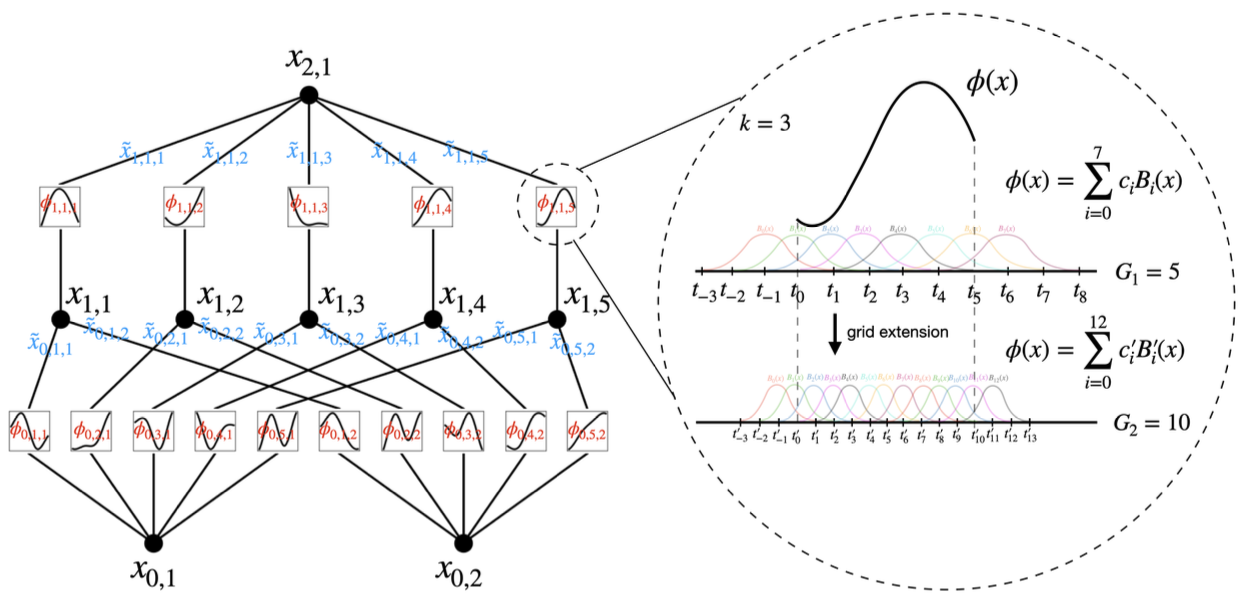
\includegraphics[width=\textwidth,keepaspectratio]{figures/KAN架構.png}
    \end{figure}
\end{frame}

\begin{frame}
    \frametitle{Kolmogorov–Arnold Network簡介}
    \centering
    \textbf{Kolmogorov-Arnold Representation theorem簡介}\\[0.5cm]
    \begin{itemize}
    \item 提出者:Andrey Kolmogorov, Vladimir Arnold
    \item 內容:針對任意有界區間 $[0,1]^n$ 上的連續函數 $f(x_1,\dots,x_n)$,\\\hspace*{3em}該定理保證:
      \begin{equation*}\label{eq:kat}
        f(x_1,\dots,x_n)
        \;=\;
        \sum_{q=1}^{2n+1}
        \Phi_q\Bigl(\,\sum_{p=1}^n \varphi_{q,p}(x_p)\Bigr)
      \end{equation*}
    \item 其中:
      \begin{itemize}
        \item $\varphi_{q,p}:\,[0,1]\to\mathbb{R}$ 為一維連續函數,作用於單一變量 $x_p$
        \item $\Phi_q:\mathbb{R}\to\mathbb{R}$ 為一維連續函數,作用於所有 $\varphi_{q,p}(x_p)$ 的加總結果
      \end{itemize}
  \end{itemize}
\end{frame}

\begin{frame}
    \frametitle{Kolmogorov–Arnold Network簡介}
    \centering
    \textbf{Kolmogorov–Arnold Networks 優勢}\\[0.5cm]
    \begin{itemize}
        \item 效能優勢:
        \begin{itemize}
            \item 小規模AI任務中,參數量更少
            \item 比MLP擁有更高精度
            \item 更快的泛化縮放律
        \end{itemize}
        \item 可解釋性:
        \begin{itemize}
            \item 激活函數可視化
            \item 可逐層稀疏修剪
            \item 適用於(準)符號回歸與科學發現
        \end{itemize}
        \item 應用優勢:
        \begin{itemize}
            \item 可用於PDE求解(PINN框架)
            \item 連續學習中能有效避免遺忘現象
            \item 結合樣條高精度與MLP組合結構
        \end{itemize}
    \end{itemize}
\end{frame}

\begin{frame}
    \frametitle{Kolmogorov–Arnold Networks實作}
    \begin{figure}
        \centering
        \begin{minipage}{\textwidth}
            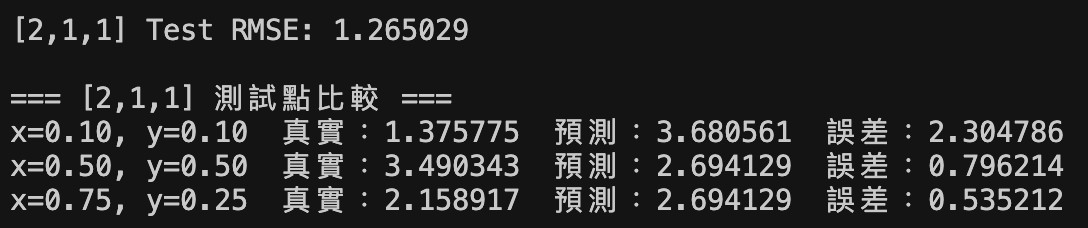
\includegraphics[width=1\textwidth,height=0.4\textheight,keepaspectratio]{figures/211_3.jpg}
            \centering
            \caption*{$\blacktriangle$ [2,1,1] 測試點比較}
        \end{minipage}
        
        \vspace{0.5em}
        
        \begin{minipage}{\textwidth}
            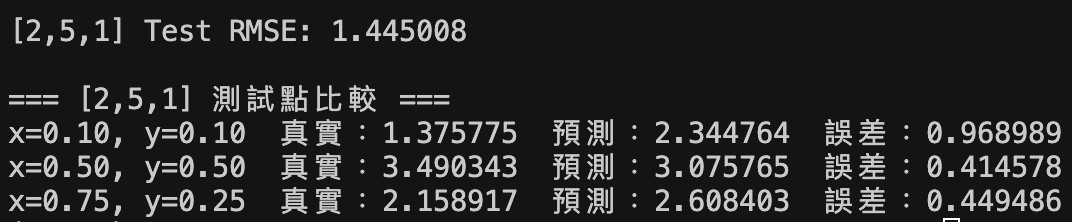
\includegraphics[width=1\textwidth,height=0.4\textheight,keepaspectratio]{figures/251.jpg}
            \centering
            \caption*{$\blacktriangle$ [2,5,1] 測試點比較}
        \end{minipage}
    \end{figure}
\end{frame}

\begin{frame}
    \frametitle{Kolmogorov–Arnold Networks實作}
    \begin{figure}
        \centering
        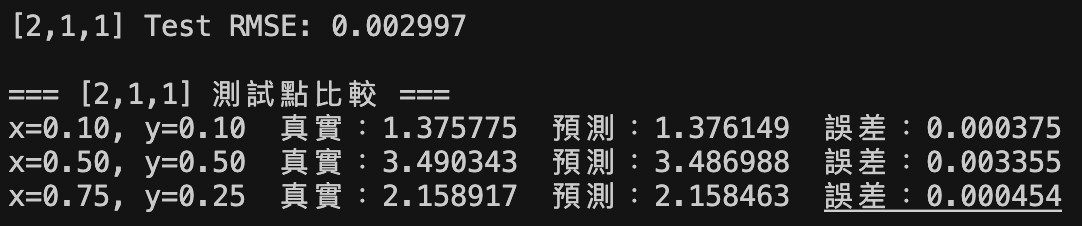
\includegraphics[width=1\textwidth,height=0.4\textheight,keepaspectratio]{figures/211比較2.jpg}
        \centering
        \caption*{$\blacktriangle$ [2,1,1]測試點比較2}
    \end{figure}
\end{frame}

\begin{frame}
    \frametitle{Kolmogorov–Arnold Networks實作}
    \begin{figure}
        \centering
        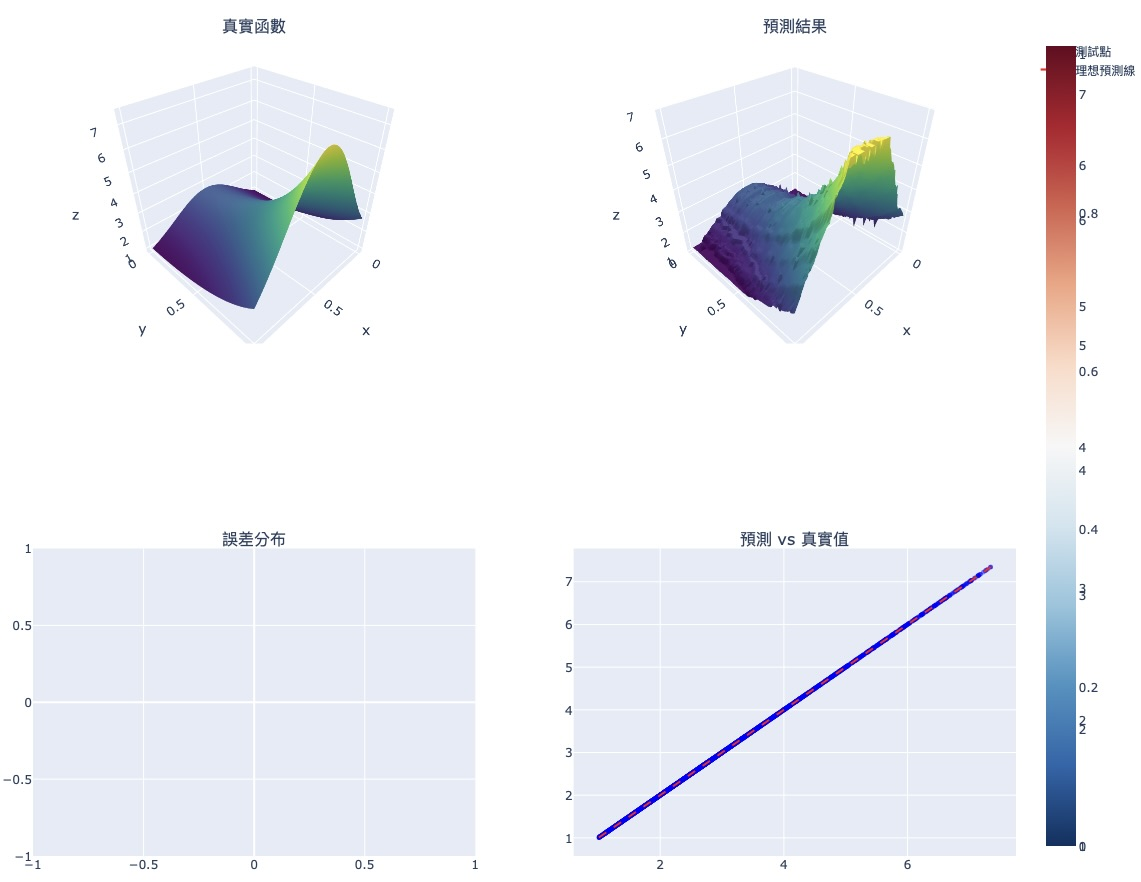
\includegraphics[width=0.75\textwidth,keepaspectratio]{figures/211比較2視覺化.jpeg}
        \caption*{$\blacktriangle$ [2,1,1]測試點比較2-視覺化}
    \end{figure}
\end{frame}

\begin{frame}
    \frametitle{Kolmogorov–Arnold Networks實作}
    \begin{figure}
        \centering
        \begin{minipage}{\textwidth}
            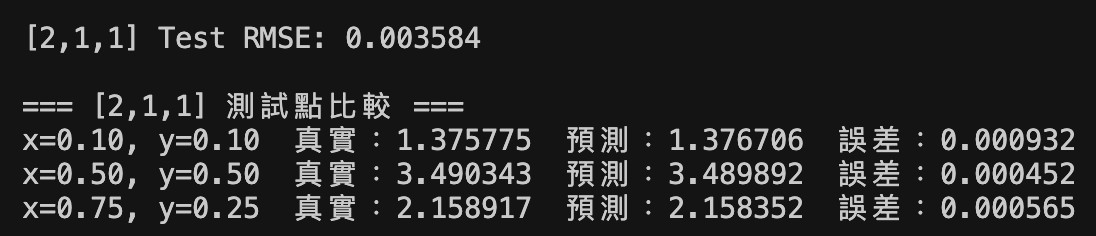
\includegraphics[width=0.9\textwidth,height=0.5\textheight,keepaspectratio]{figures/211比較1.jpg}
            \centering          
        \end{minipage}
        
        \begin{minipage}{\textwidth}
            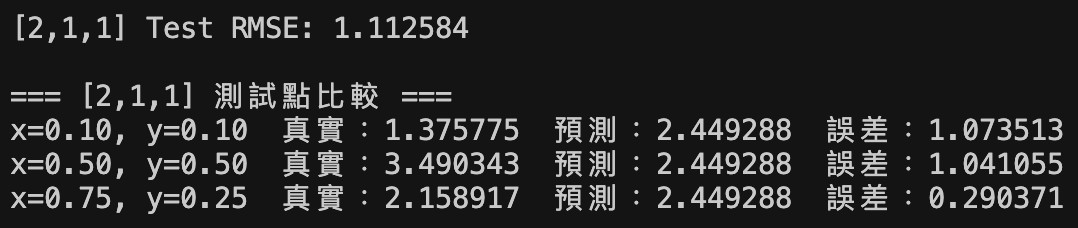
\includegraphics[width=0.9\textwidth,height=0.5\textheight,keepaspectratio]{figures/211比較6.jpg}
            \centering
        \end{minipage}

        \begin{minipage}{\textwidth}
            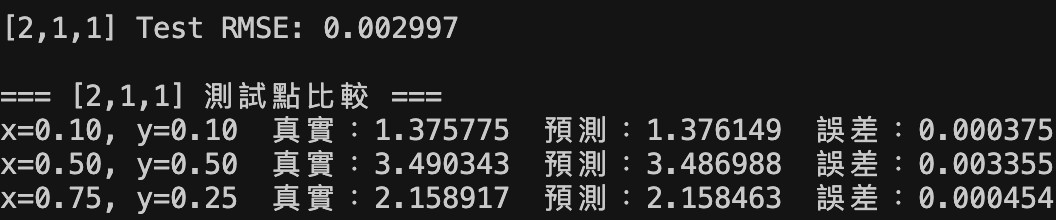
\includegraphics[width=0.9\textwidth,height=0.5\textheight,keepaspectratio]{figures/211比較12.jpg}
            \centering            
        \end{minipage}
    \end{figure}
\end{frame}

\begin{frame}{記憶模型是否能降低KAN的誤差}
  \centering
  \begin{figure}
    % 左邊圖片,寬度設成文字區的一半(約 0.48\textwidth),留點間距
    \begin{minipage}{0.49\textwidth}
      \centering
      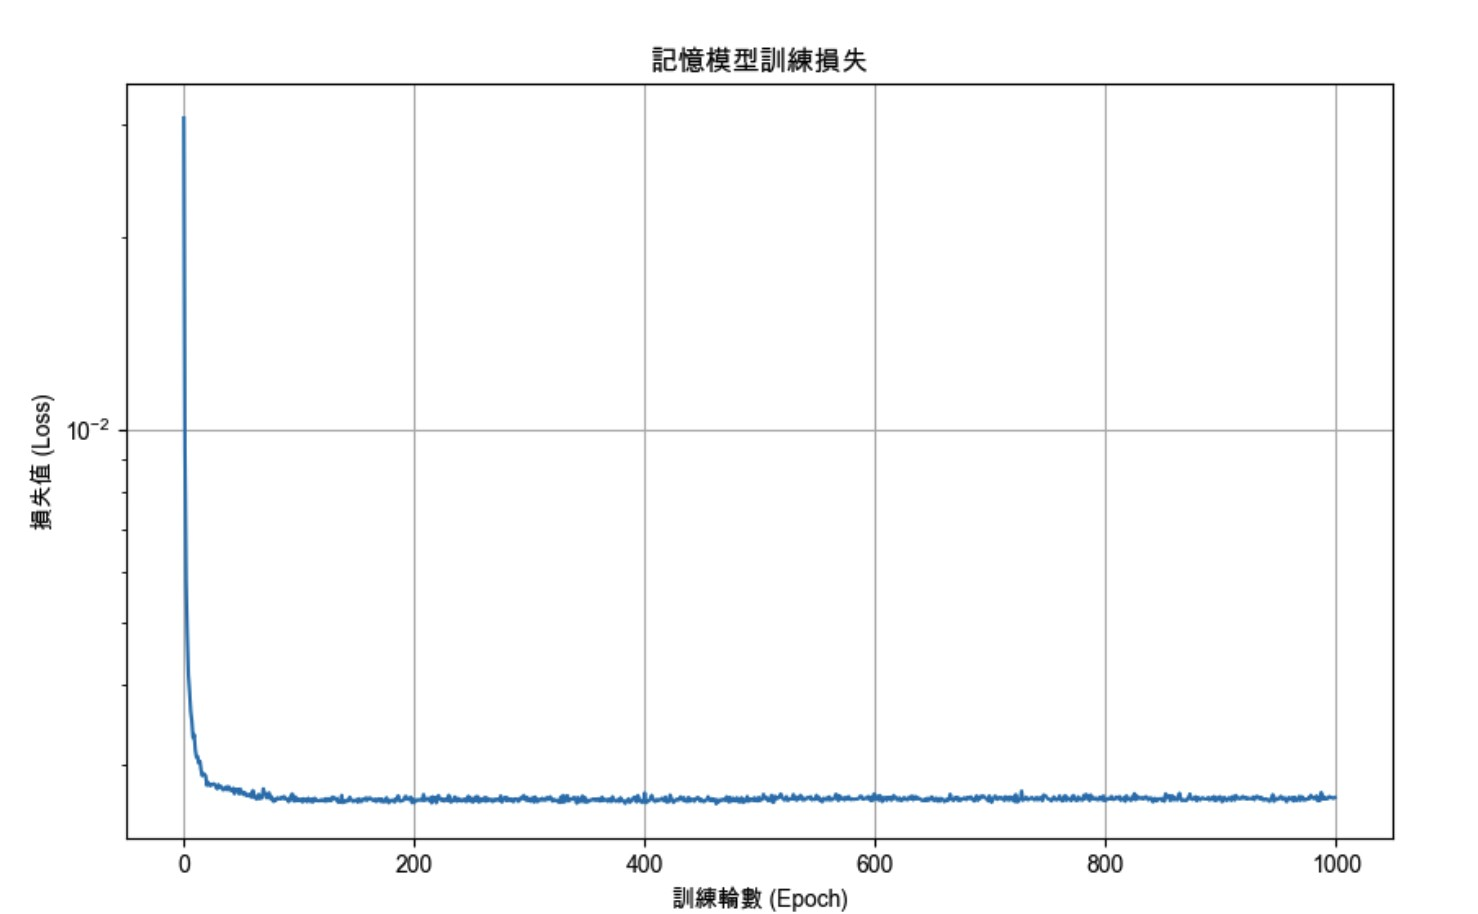
\includegraphics[width=\textwidth, keepaspectratio]{figures/記憶功能.jpg}
      \caption*{$\blacktriangle$ 記憶功能訓練結果}
    \end{minipage}%
    \hfill % 用 \hfill 讓左右兩個區塊盡量對齊留白
    % 右邊圖片,同樣寬度
    \begin{minipage}{0.49\textwidth}
      \centering
      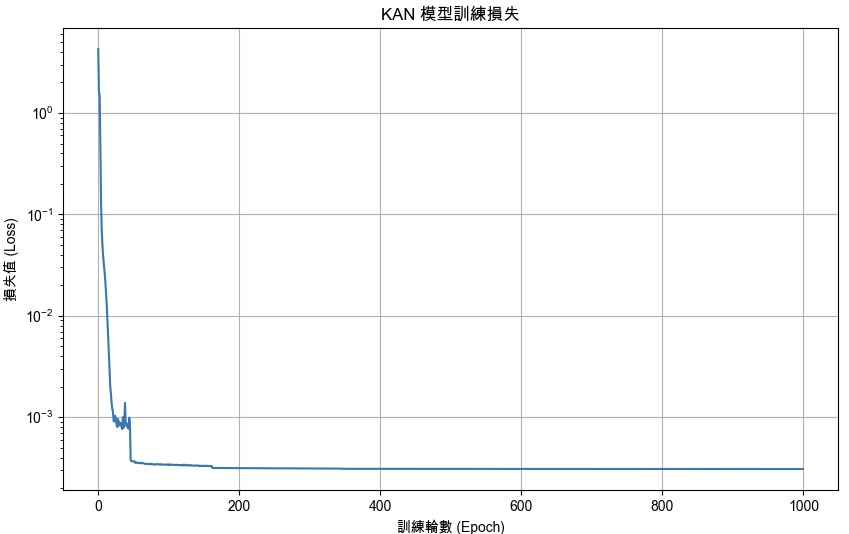
\includegraphics[width=\textwidth, keepaspectratio]{figures/kan_training_loss.jpeg}
      \caption*{$\blacktriangle$ KAN訓練結果}
    \end{minipage}
  \end{figure}
\end{frame}

\begin{frame}
    \frametitle{記憶模型能不能降低KAN的誤差}
    \begin{figure}
        \centering
        \begin{minipage}{\textwidth}
            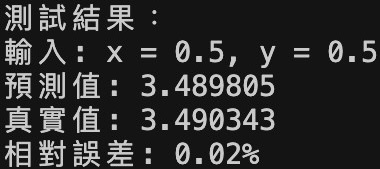
\includegraphics[width=0.8\textwidth,keepaspectratio]{figures/增加記憶功能後的結果.jpg}
            \centering
            \caption*{$\blacktriangle$ 增加記憶功能後的結果數據}
        \end{minipage}
    \end{figure}
\end{frame}

\begin{frame}
    \begin{center}
        \Huge\textbf{謝謝大家}
        
        \vspace{1em}
        \Large 報告結束
    \end{center}
\end{frame}

\end{document} 